%%%%%%%%%%%%%%%%%%%%%%%%%%%%%%%%%%%%%%%%%%%%%%%%%%%%
\section{Informed Plan Selection}\label{sec:coverage}
%%%%%%%%%%%%%%%%%%%%%%%%%%%%%%%%%%%%%%%%%%%%%%%%%%%%

%In this section, we extend our BDI learning so as to include a confidence test
%within the plan selection mechanism itself. More concretely, in the new approach,
%instead of using the stability measure to ensure that we only record results that
%we are confident in, we instead modify our plan selection procedure to take into
%account of how confident we are in the current \dt.
% %
Our new approach relies on the idea that confidence in a plan's
\dt increases as more of the possible choices below the plan
in the goal-plan structure are explored.
% %
%Note that while the stability mechanism ensures that failure information is
%\emph{not recorded} against a \dt until the corresponding goal-plan
%structure is adequately explored; the new approach instead influences how the
%\dt is \emph{used} at plan selection time.
This set of all potential execution paths
below the plan in the hierarchy is easily computed offline from the static goal-plan structure.
% %
Intuitively, a plan's \dt is more \textit{informed} for a world
state if it is based on a larger number of choices having been
explored in that state.
%accounts for a larger number of the plan's choices in that state.
% %
We say that a plan has a higher degree of \emph{coverage} as more of its
underlying choices are explored and accounted for in the
corresponding \dt.
% %

Technically, given a \dt $T$ for a plan, we define its coverage for the world state $w$ as 
$c_T(w) \in [0,\ldots,1]$.
% %
Initially, prior to world state $w$ being first observed, the plan's coverage is 
$c_T(w)=0$ i.e. the agent has no confidence in the likelihood of success estimated by $T$ for $w$. As the
different ways of executing the plan in the world state $w$ are explored, the value of
$c_T(w)$ approaches $1$. When all choices have been tried, $c_T(w)=1$ and the
agent may rely fully on the \dt estimation of success.
% %
In this way, coverage provides a confidence measure for the \dt classification.

We now construct a probabilistic plan selection function that includes the coverage-based confidence measure.
% %
Formally, we define the plan selection weight $\Omega'(w)$ as a function of the \dt determined success expectation $p_T(w)$ and the degree of coverage $c_T(w)$:
%
\begin{equation*}\label{eqn:coverage}   
\Omega'_T(w) = 0.5 + \left[  c_T(w) *  \left( p_T(w) - 0.5 \right)  \right]
\end{equation*}
	
	
Initially the selection weight of the plan for a previously unseen world state $w$ takes the default value of $0.5$.
% %
Over time, as the various execution paths below the plan are tried in $w$, it's coverage increases 
and the selection weight approaches the true value estimated by the plan's \dt.


%Regarding how the coverage degree is calculated at every point, we should make
%the following two observations.
% %
Each time a plan execution result is recorded, the coverage
$c_T(w)$ for a world $w$ is calculated and stored.
% %
It requires, in principle, $\tau \times |S|$ \emph{unique} executions of
a plan for it to reach \emph{full} coverage, where $\tau$ is the total number of
choices below the plan and $|S|$ is the number of possible worlds. Practically,
however, it takes significantly less since choices below a plan are effectively
an AND/OR tree, and each time an AND node fails, the subsequent
nodes are not tried and are counted as covered for the world in question.
% %
Also, a plan is generally not executed in every world state, so in
practice it will only need to be assessed in the subset of the world
states that is relevant to it.
%Moreover, since plans are typically executed in the context of other plans
%(e.g., the plan to check-in is always executed after a plan to go to the
%airport), it would not be necessary to account for the whole world space, but
%only for its subset that is relevant for the plan.

\medskip We are now ready to revisit the two
learning approaches \CL\ and \BUL\ from the previous section but using the modified
selection weighting based on coverage. We will refer to the new agents as \CLSELB\
and \BULSELB, respectively.
% %
Similarly, $\CLSELA$ and $\BULSELA$ correspond to the agents using
the \emph{original} selection weighting that only uses 
its \dt success expectation $\Omega_T(w) = p_T(w)$.


Our first observation is that the $\BULSELA$ and $\BULSELB$ approaches show similar performance.
% %
This is not surprising, as the stability test performed by these agents at each
plan node inherently results in close to full coverage. Indeed, for a plan to become
``stable,'' the agent needs to (substantially) explore all possible  ways of
executing it. The stability check, then, effectively reduces
$\Omega'_T(w)$ to $\Omega_T(w)$. 
So for simplicity we will not give a further account of the $\BULSELB$ approach in this section.



We now focus on the \CL\ approach.
% %
For the \CL-favouring structure $\T_1$, we find that the performance of $\CLSELB$ matches that
of $\CLSELA$ reported earlier in Figure~\ref{fig:T1_result}.
% %
Similarly, for the balanced structure $\T_3$ where previously both \CL\ and
\BUL\ performed equally well, the performance of $\CLSELB$
was the same as that reported for $\CLSELA$ earlier in Figure~\ref{fig:T3_result}.
% %
Thus, for the cases where $\CLSELA$ was performing reasonably well, the new $\CLSELA$ approach maintains comparable performance.

\begin{figure}[t]
\begin{center}
%!TEX root = ../dsingh-aamas10.tex
\begin{tikzpicture}[x=0.00276cm,y=5cm]
    % Draw the axes and grid lines
    \draw[-] (0,0) -- (0,1) -- (3000,1) -- (3000,0) -- cycle; 
    \draw[-,thin, dotted, ystep=0.2, xstep=3000] (0,0) grid (3000,1);
    \foreach \x in {500, 1500, 2500}  \draw [-,xshift=0](\x,4pt) -- (\x,-1pt);
    \foreach \y in {0.0,0.2,0.4,0.6,0.8,1.0}  \draw [-,yshift=0](4pt,\y) -- (-1pt,\y);
    \foreach \x/\xtext in {500/500, 1500/1500, 2500/2500} \node at (\x,0) [below] {$\xtext$};
    \foreach \y/\ytext in {0.0,0.2,0.4,0.6,0.8,1.0}  \node at (0,\y) [left] {$\ytext$};
    \node at (0,1.1) {Success};
    \node at (2700,0.15) {Iterations};
    \draw[-,red] plot[mark=x,mark size=4,mark options={color=red}] 
			file {figs/data/test05v3gm.CC.tikzdata};
    \draw[-,thin,densely dashed,black] plot[mark=x,mark size=4,mark options={color=black}] 
			file {figs/data/test05v3gm.CP.tikzdata};
    \draw[-,thin,densely dashed,black] plot[mark=o,mark size=2,mark options={color=black}] 
			file {figs/data/test05v3gm.SP.tikzdata};
    % Also draw the expected convergence: 0.9^8 actions=0.43046
    \draw[dashed,-,yshift=0](0,0.43046) -- (3000,0.43046);

\end{tikzpicture}

\caption{Performance of $\CLSELB$ (solid crosses) in structure $\T_2$ compared against
the earlier results for $\CLSELA$ and $\BULSELA$ (both in dotted grey).}
\label{fig:T2_result2}
\end{center}
\end{figure}

The benefit of the coverage-based approach is apparent, though, when one considers the goal-plan
structure $\T_2$ in which the $\CLSELA$ used to perform poorly (cf. Figure
\ref{fig:T2_result}).
% %
Here the $\CLSELB$ approach showed a dramatic improvement over
$\CLSELA$. Figure \ref{fig:T2_result2} shows this change with the results
for the new approach to plan selection $\BULSELB$ and $\CLSELB$ superimposed over
the original results from Figure \ref{fig:T2_result}.
% %
The reason why the new plan selection mechanism improves the \CL\ learning scheme
is that even though the success estimation $p_T(w)$ for a given plan $P_i$ would still be low
initially (remember that \CL, in contrast with \BUL, would record all initial
failure outcomes for $P_i$), the agent would not be very confident in such
estimation until the plan's coverage increases and therefore the selection weight 
$\Omega'_T(w)$ will initially bias more towards the default weight of $0.5$.
In other words, the false negative outcomes collected by the agent for plan $P_i$ would not be considered
so seriously due to low plan coverage. As full coverage is approached, one would
expect the agent to have discovered the success execution encoded in $P_i$.


Even more interesting is the the impact of the new plan selection mechanism on
agents that work with an applicability threshold i.e. agents that may not
select a plan if it is deemed unlikely to succeed. 
%
Here, the original $\CLSELA$ approach fails as it collects many negative experiences early on, causing it to fall below the selection threshold quickly. 
For $\CLSELB$, even if a plan is deemed with very low expectation of success, if it
has not been substantially ``covered'' then its selection weight would be biased towards the
default value of $0.5$. So provided that the applicability threshold is always set lower that the default plan selection weight (also the case for \BUL), then $\CLSELB$ is able to find the solution.
%%
Figure~\ref{fig:performance-applicability} shows the $\CLSELB$ performance in goal-plan structure $\T_2$ for an applicability threshold of $0.2$.


\begin{figure}[t]
   \centering
   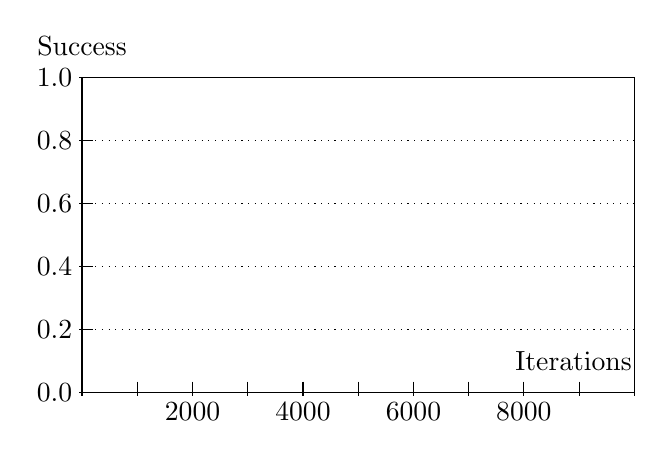
\begin{tikzpicture}[x=0.0007cm,y=4cm]
    % Draw the axes and grid lines
    \draw[-] (0,0) -- (0,1) -- (10000,1) -- (10000,0) -- cycle; 
    \draw[-,thin, dotted, ystep=0.2, xstep=10000] (0,0) grid (10000,1);
    \foreach \x in {0,1000,...,10000}  \draw [-,xshift=0](\x,4pt) -- (\x,-1pt);
    \foreach \y in {0.0,0.2,0.4,0.6,0.8,1.0}  \draw [-,yshift=0](4pt,\y) -- (-1pt,\y);
    \foreach \x/\xtext in {2000/2000, 4000/4000, 6000/6000, 8000/8000} \node at (\x,0) [below] {$\xtext$};
    \foreach \y/\ytext in {0.0,0.2,0.4,0.6,0.8,1.0}  \node at (0,\y) [left] {$\ytext$};
    \node at (0,1.1) {Success};
    \node at (8900,0.1) {Iterations};
    \draw[-] plot[mark=square,mark size=2,mark options={color=black}] 
			file {data/testMultiSolutionsR.CC.tikzdata};
    \draw[-,thin,densely dashed,gray] plot[mark=triangle,gray,mark size=3,mark options={color=gray}] 
			file {data/testMultiSolutionsR.CP.tikzdata};
    \draw[-] plot[mark=diamond,mark size=3,mark options={color=black}] 
			file {data/testMultiSolutionsR.SC.tikzdata};
    \draw[-,thin,densely dashed,gray] plot[mark=o,gray,mark size=2,mark options={color=gray}] 
			file {data/testMultiSolutionsR.SP.tikzdata};

\end{tikzpicture}

   \caption{Performance of $\CLSELB$ (solid crosses) compared against $\CLSELA$ and $\BULSELA$ (both in dotted grey) in structure $\T_2$ using an applicability threshold of $0.2$.}
   \label{fig:performance-applicability}
\end{figure}

\Omit{
Finally, we point out that agents based on the new coverage-based plan selection
scheme will be able to realize when the optimal solution for a goal has been
reached before the agents based on the original scheme.
% %
This happens because, by using the coverage degree to calculate the final weight
of a plan for a goal, the system is both looking for successful paths while
maximizing    the uniform exploration of the agent's plan library.
% %
So, for example, since $P$ is more ``complex'' than $P_i'$ in in structure $\T_2$
(Figure~\ref{fig:T2}), an agent based on the $\Omega'$ weighting function, will
tend to give more execution chances to the former in order to achieve a more
uniform exploration of the options for goal $G$.
}

The above results show that the coverage-based confidence weighting
can improve the performance of the \CL\ approach in those
cases where it performed poorly due to false negative experiences,
i.e., failure runs for a plan that includes successful executions.
%

Furthermore coverage provides a flexible mechanism for tuning agent 
behaviour depending on application characteristics. Consider equation $\Omega'_T(w)$ with the coverage term modified to $c_T(w)^{1/\alpha}$ where $\alpha$ determines the agent behaviour. Then, as $\alpha \approx 0$, $\CLSELB$ will behave more
like $\BULSELA$: $c_T(w)^{1/\alpha}$ transitions directly from $0$
to $1$ when $c_T(w)$ reaches $1$ (and remains zero otherwise).
% %           
On other hand, when $\alpha \approx \infty$, $\CLSELB$ will behave more
like the $\CLSELA$: $c_T(w)^{1/\alpha}$ transitions from $0$ to $1$ faster and
$\Omega'(w) \approx p_T(w)$.
%
With $\alpha=1$ we get our initial equation.

Finally, we note that coverage-based selection weights encourage the agent to
explore all available options. This further ensures that all solutions are systematically 
found, allowing the agent to decide which solution is optimal. For some domains
this may be an important consideration.



\Omit{
The above results are significant in that they suggest that the alternative plan
selection mechanism, which includes a confidence test based on the notion of plan
coverage, can substantially improve the performance of the \CL\ approach in those
cases where it performed poorly due to false negative experiences, i.e., failure
runs for a plan that includes successful executions.
% %
The main point here is that \CLSELB\ provides a \emph{middle ground} between
\CLSELA\ and \BULSELA. In fact, one can easily extend the plan weight formula to
bias the architecture towards one of the two extremes, namely: (The
original formula is obtained when $\alpha=1$.)
% %
\begin{equation*}\label{eqn:coverage*}   
\Omega'_T(w) = 0.5 + \left[  c_T(w)^{1/\alpha} *  \left( p_T(w) - 0.5 \right) 
\right].
\end{equation*}

\noindent Hence, when $\alpha \approx 0$, the \CLSELB\ scheme will behave more
like a \BULSELA-based system: $c_T(w)^{1/\alpha}$ transitions directly from $0$
to $1$ when $c_T(w)$ reaches $1$ (and it remains zero otherwise).
% %
On other hand, when $\alpha \approx \infty$, the \CLSELB\ scheme will behave more
like the \CLSELA: $c_T(w)^{1/\alpha}$ transitions from $0$ to $1$ faster and
$\Omega'(w) \approx p_T(w)$.
% %

Putting it altogether, all the above suggests that the \CLSELB\ learning
approach is most adequate to address the problem we are concerned on, since it
is simpler and more flexible than the alternative ones.
}



% Nonetheless, it should be noted that in our problem there is indeed the usual a
% intrinsic trade-off between exploration and execution success.





% \bigskip\bigskip\bigskip
% \textbf{move to discussion??}
% Since the
% coverage $c_T(S)$ in Equation \ref{eqn:coverage} is simply a
% confidence measure, then the way it is \textit{used} will determine
% the weighting of the confidence in the final plan selection
% probability $p'_T(w)$. For instance we could replace $c_T(S)$ in
% Equation \ref{eqn:coverage} with $c_T(S)^{1/b}$ where $b$ is the
% weighting (and $b=1$ gives us the original Equation
% \ref{eqn:coverage}). Then adjusting $b \rightarrow 0, (0 \ne b < 1$)
% we get more \BUL+$E$-like performance, while adjusting $b \rightarrow
% \infty (b > 1)$ will result in more \CL+$E$-like performance. In fact,
% an improved agent could reference the (static) goal-plan tree
% structure at runtime and adjust $b$ automatically based on the offline
% compiled knowledge of which approach works better for which tree
% topology. 
% % This extension is left as a future implementation exercise. 
% 
% We noted earlier in Section \ref{sec:experiments} that plan execution
% in real systems is often not cost-free, so presumably the agent would
% not execute a plan with too low a probability of success. We also show
% that such deliberation does not favour \CL\ but does \BUL. It is clear
% that choosing not to execute a plan below a threshold probability of
% failure would also hurt the \CL+$E'$ configuration (though
% not as much as \CL+$E$). For such systems, we suggest that the
% weighting $b$ be used to get the preferred \BUL-like performance. 


